\chapter{Research Approach}\label{Chap:ResearchApproach}

The ELM model, as demonstrated in previous research \cite{salam2021earthquake, asim2017earthquake}, offers notable advantages by running faster than classical ANNs and maintaining high accuracy. Moreover, the recurrent unit layer in the Echo State Network (ESN), as supported by studies like \cite{cucchi2022hands, bianchi2020reservoir}, provides an efficient approach for feature data representation in supervised learning models without the need for extensive training.

The combination of the ELM and ESN models offers a compelling approach. ELM is recognized for its efficient, high-speed performance and the ability to maintain accuracy. Meanwhile, the recurrent unit layer of the Echo State Network (ESN) stands out by representing feature data effectively for supervised learning models without necessitating extensive training.

%P5. research app
This study proposes a multi-channel echo state extreme learning machine called Multi ES-ELM. This model combines an Extreme Learning Machine (ELM) and the Echo State Network (ESN). ELM is a neural network that uses only a single hidden layer and does not require backpropagation or multiple retrainings, as is typical with conventional neural network models. 

Consequently, ELM training is significantly faster than deep learning, making it suitable for EEW systems that constantly receive new datasets and need to train with new data instantly. 

However, the parameters used in ELM are typically chosen randomly, which can impact the model's accuracy. To increase ELM's accuracy, the Echo State Network (ESN) model, a type of Reservoir Computing (RC), is incorporated. The ESN is used to adjust the parameters used in ELM. Thus, it's possible to improve the accuracy of the EEW with our proposed model while maintaining fast training times. 

The proposed model is designed to train with multiple time series data, given that seismic wave data consists of three data channels. The proposed model performs nearly as well as the CNN model but requires fewer resources.

%P6. advantage paragraph
The ESN model is small, needs low computer resources to train, and is combined with the ELM. This reason leads to the ability to retrain the Multi ES-ELM frequently. Thus, the model reduces the training model's cost while building a precise system to protect against danger from earthquake events.

This section is divided into three parts that overview the data, the method for training, and the Multi-channels Echo State Extreme Learning Machine (Multi ES-ELM) model. The section \ref{sec:data} explains the input data $X$ and the output data $Y$ used to train in the proposed model. The section \ref{sec:training} shows how to train Extreme Learning Machine via pseudo inverse.  The \ref{subsec:multi model} part overviews the proposed model's structure and shows how to use the Multi-Channel ESELM to train the model. The code for my model is available on GitHub \footnote{https://github.com/OrnlyP63/multi-esn-eews}.

% \begin{table}
% \centering
% \caption{Symbol and Notation}
% \label{table:notation}
% \setlength{\tabcolsep}{3pt}
% \begin{tabular}{|c|p{350pt}|}
% \hline
% Symbols& Meaning \\
% \hline
% $I$ & Identity matrix\\

% $N$ & Number of samples in a dataset \\

% $\lambda$ & Number of internal units of the ESN layer \\

% $C$ & Number of channels of signal data \\

% $M$ & Number of class of data \\

% $T$ & Period length of signal data\\

% $\mathcal{S}$ & A signal matrix of size $T\times C$\\

% $s_t$ & A signal point at time $t$\\

% $X$ & A tensor dataset of signal data of size $N\times T\times C$\\

% $Y$ & A matrix of label of size $N \times 2$\\

% $h_t$ & A hidden state at time $t$\\

% $H$ & A Hidden matrix\\

% $\mathcal{H}$ & List of hidden matrix $[H_1;H_2;\cdots;H_N]$ \\

% $R$ & Ridge Embedding of $H$\\

% $\mathcal{R}$ & List of Ridge Embedding $[R_1;R_2;\cdots;R_N]$\\

% $n$ & The time steps for embedding\\

% $W_{input}$ & An input matrix of the ESN of size $\lambda\times C$\\

% $W_{h}$ & An internal units matrix of the ESN of size $\lambda\times \lambda$\\

% $W_{output}$ & An output matrix of the Multi-ESELM of size $2 \times\lambda$\\

% $g(\cdot)$ & A Non-linear function or hidden neuron activation function\\

% $\tanh(\cdot)$ & A tangent function\\

% $flatten(\cdot)$ & A flatten function is a function to flat a vector or a matrix to a row vector.\\

% $l$ & Number of hidden units of ELM\\

% $\mathbf{A}$ & Input data of ELM\\ 

% $\mathbf{G}$ & A hidden layermatrix of ELM\\

% $\mathcal{B}$ & An outpit weight of ELM\\

% $A$ & A coefficient vector of solution of a least square problem\\

% $B$ & A bias vector of solution of the least square \\
% \hline

% % \multicolumn{2}{p{251pt}}{footnote letters. }\\
% \end{tabular}
% \end{table}

\section{Data preparation for input data and label data}\label{sec:data}
The ground acceleration data is collected from the earthquake station. Figure ~\ref{fig:input-data} shows the input data is the ground acceleration of the initial P-wave (500 samples of a P-wave), which consists of three axes: $NS,$ $EW,$ and $Z$ \cite{chiang2022neural, jozinovic2020rapid}. Also, the 500 samples of a P-wave is the best sample size for the convolutional neural network model from \cite{chiang2022neural}. Consider the observation signal $S_i$ at time $t$ is denoted as $[NS_t, EW_t, Z_t]^\top$. The input data for the Multi ES-ELM model is the multivariate time series data and the $i-th$ input data can be represented by the matrix.
\begin{equation*}
    \mathcal{S}_i 
% = [s_1, s_2, \cdots, s_T]
=
\begin{bmatrix}
NS_{1} & NS_{2} & \cdots & NS_{T}\\
EW_{1} & EW_{2} & \cdots & EW_{T}\\
Z_{1} & Z_{2} & \cdots & Z_{T}\\
\end{bmatrix}_i\in \mathbb{R}^{3\times T}
\end{equation*}
The Signals dataset is defined by the tensor
\begin{equation*}
 X = 
\begin{bmatrix}
\mathcal{S}_{1}\\
\mathcal{S}_{2}\\
\vdots\\
\mathcal{S}_N
\end{bmatrix} \in \mathbb{R}^{N\times 3\times T}
\end{equation*}
where $T$ is the number of samples of the initial P-wave and $N$ is the number of signal data.    

The label $y_i$ of the data $\mathcal{S}_i$ is the peak ground acceleration (PGA) of the seismic signal. The labels of the dataset are encoded by one hot encoder. By the setting from \cite{chiang2022neural}, if the PGA of the signal $\mathcal{S}_i$ is less than $80Gal$ then 
$$y_i = \begin{cases}
    [1, 0], & \text{Not warning}\\
    [0, 1], & \text{Warning}.
\end{cases}$$
Moreover, the matrix of labels is expressed by
% $$y_i = \text{PGA of i-th input data}$$
\begin{equation*}
Y = 
\begin{bmatrix}
y_1\\
y_2\\
\vdots\\
y_N\\
\end{bmatrix}\in\mathbb{R}^{N\times 2}
\end{equation*}
where $T$ is the time instants and $N$ is the number of samples.\\ 

\section{Training Method}\label{sec:training}

In 2006, Huang \cite{huang2006extreme} studied and expanded  extreme learning machine
by the following model: for any $N$ distinct samples  $(x_i,t_i)$ where $x_i=[x_{i1}, x_{i2},...,x_{in}]^T\in\mathbb{R}^n$ and $t_i=[t_{i1}, t_{i2},...,t_{im}]^T\in\mathbb{R}^m$, standard SLFNs with $\tilde{N}$  hidden nodes and activation function $g(x)$ are mathematically modeled as\\
% \begin{figure}[h]
% \centering
% \includegraphics[width=0.75\textwidth]{sl}
% \end{figure}
\begin{align}
&\sum\limits_{i=1}^{\tilde{N}}\beta_ig(w_i\cdot x_j+b_i)=\hat y_j, 
\end{align}
where $j=1,...,N$ and $w_i=[w_{i1}, w_{i2},...,w_{in}]^T$ is the weight vector connecting the $i$-th hiden node and the input nodes, $\beta_i=[\beta_{i1}, \beta_{i2},...,\beta_{im}]^T$ is the weight vector connecting the $i$-th hidden node and the output nodes, and $b_i$ is the threshold of the $i$-th hidden node, $w_i\cdot x_j$ denotes the inner product of $w_i$ and $x_j$. The standard SLFNs with $\tilde{N}$ hidden nodes with activation function $g(x)$ can approximate these $N$ samples with zero error means $\sum\limits_{j=1}^{\tilde{N}}\|\hat y_j-y_j\|_2=0$, where $\|\cdot\|_2$ is defined by $\|x\|_2=\sqrt{\sum\limits_{i=1}^n|x_i|^2}$. That is there exist $\beta_i, w_i$ and $b_i$ such that
\begin{align}
&\sum\limits_{i=1}^{\tilde{N}}\beta_ig(w_i\cdot x_j+b_i)=y_j, j=1,...,N
\end{align}
The above $N$ equations can be written compactly as 
\begin{align}
H\beta=Y,
\end{align}
where
\begin{align}
H &=\begin{bmatrix}
g(w_1\cdot x_1+b_1) & \cdots & g(w_{\tilde{N}}\cdot x_1+b_{\tilde{N}})\\
\vdots & \ddots & \vdots\\
g(w_1\cdot x_N+b_1)  & \cdots & g(w_{\tilde{N}}\cdot x_N+b_{\tilde{N}}) 
\end{bmatrix}_{N\times\tilde{N}},\\
\beta&=
\begin{bmatrix}
\beta_1^T\\
\vdots\\
\beta_{\tilde{N}}^T
\end{bmatrix}_{\tilde{N}\times m}
\text{and}~~~~
Y=\begin{bmatrix}
y_1^T\\
\vdots\\
y_N^T
\end{bmatrix}_{N\times m}.
\end{align}
To train an SLFN, one may wish to find specific $\hat{W}_i,\hat{b}_i,\beta$ where $i=1,...,\tilde{N}$ such that 
\begin{align}
\min_{\beta}\|H\beta-Y\|_2=\min_{w_i,b_i,\beta}\|H(w_1,...,w_{\tilde{N}},b_1,...,b_{\tilde{N}})\beta-Y\|_2
\end{align}
which is equivalent to minimizing the cost function
\begin{equation}
E=\sum\limits_{j=1}^N\left(\sum\limits_{i=1}^{\tilde{N}}\beta_ig(w_i\cdot x_j+b_i)-y_j\right)^2.
\end{equation}
For fixed input weights $w_i$ and the hidden layer biases $b_i$ to train an SLFN is simply equivalent to finding a least squares solution $\tilde{\beta}$ of the linear system $H\beta=T$:
\begin{equation}
\min_{\beta}\|H(\hat{w}_1,...,\hat{w}_{\tilde{N}},\hat{b}_1,..., \hat{b}_{\tilde{N}})\hat{\beta}-Y\|_2^2=\min_{w_i,b_i,\beta}\|H(w_1,...,w_{\tilde{N}},b_1,...,b_{\tilde{N}})\beta-Y\|_2^2.
\end{equation}
The smallest norm least squares solution of the above linear system is 

\begin{align}
\hat{\beta}=H^{\dag}T, 
\end{align}

where $H^{\dag}$ is the Moore-penrose generalized inverse of matrix $H$.

The training method that is used in the training part of the Multi ES-ELM model is the pseudo-inverse method from Extreme Learning Machine (ELM).  The ELM's structure can be written by the matrix.
\begin{equation*}
    H\hat\beta = \hat Y
\end{equation*}

where 
% \begin{equation*}
%     \mathbf{G} = 
% \begin{bmatrix}
% g(a_1\cdot w_1 + b_1) & \cdots & g(a_1\cdot w_l + b_l)\\
% \vdots & \ddots & \vdots\\
% g(a_N\cdot w_1+b_N) & \cdots & g(a_N\cdot w_l + b_l)\\
% \end{bmatrix}\\
% \end{equation*}
\begin{equation*}
    \hat\beta = 
    \begin{bmatrix}
    \beta_1\\
    \vdots\\
    \beta_m
    \end{bmatrix}\quad \text{and}\quad
    \hat Y = 
    \begin{bmatrix}
    \hat y_1\\
    \vdots\\
    \hat y_N
    \end{bmatrix}
\end{equation*}
$g,\ \mathbf{A} = [a_1, \ldots a_N]^\top,\ \mathbf{b} = [b_1,\ldots, b_l]^\top, \mathbf{W} = [w_1,\ldots, w_l]^\top, \hat Y$ and $\beta$  are a non-linear function, input data, bias, input weight, prediction, and optimal output weight respectively.

\begin{algorithm}
  \caption{Training Extreme Learning Machine (ELM)}
  \label{elm_training_algorithm}
  \begin{algorithmic}[1]
    \renewcommand{\algorithmicrequire}{\textbf{Input:}}
    \renewcommand{\algorithmicensure}{\textbf{Output:}}
    \Require Input matrix $\mathbf{A} \in \mathbb{R}^{N \times d}$, output matrix $Y \in \mathbb{R}^{N \times k}$, activation function $g(\cdot)$
    \Ensure Input weight $\mathbf{W} \in \mathbb{R}^{d \times l}$, hidden bias $\mathbf{b} \in \mathbb{R}^{l \times 1}$, output weight matrix: $\beta \in \mathbb{R}^{l \times k}$

    \State $\mathbf{W}\gets [w_{ij}] \in \mathbb{R}^{d \times l},\  w_{ij} \sim U(-1, 1)$
    
    \State $\mathbf{b}\gets [b_{ij}] \in \mathbb{R}^{l \times 1},\  b_{ij} \sim U(-1, 1)$ 
    
    \State$H \gets g(\mathbf{A} \cdot \mathbf{W} \oplus \mathbf{b}^\top)$
    \State $H^\dagger \gets (H^\top  H)^{-1}  H^\top$
    \State $\hat{\beta} \gets H^\dagger Y$
    \State \textbf{Return} $\mathbf{W}$, $\mathbf{b}$, $\hat{\beta}$
  \end{algorithmic}
\end{algorithm}

Algorithm \ref{elm_training_algorithm} shows the method to find the optimal output weight $\hat{\beta}$ for the ELM model. $H$ is the hidden layer or learnable representation of the ELM. Furthermore, $\hat\beta$ is the trained layer (output weight) of the ELM. The ELM uses the pseudo-inverse of the $H$ matrix $(H^{\dagger})$ to find the optimal trained layer $\hat{\beta}$ in the model\cite{huang2006extreme}.
$$\hat{\beta} = H^{\dagger}Y$$
where $H^{\dagger} = (H^\top H^{-1}H^\top)$.

The $W_{output}$ of the Multi ES-ELM uses the following method to find the optimal weight $\hat{W}_{output}$. 

\begin{figure}[ht]
    \centering
    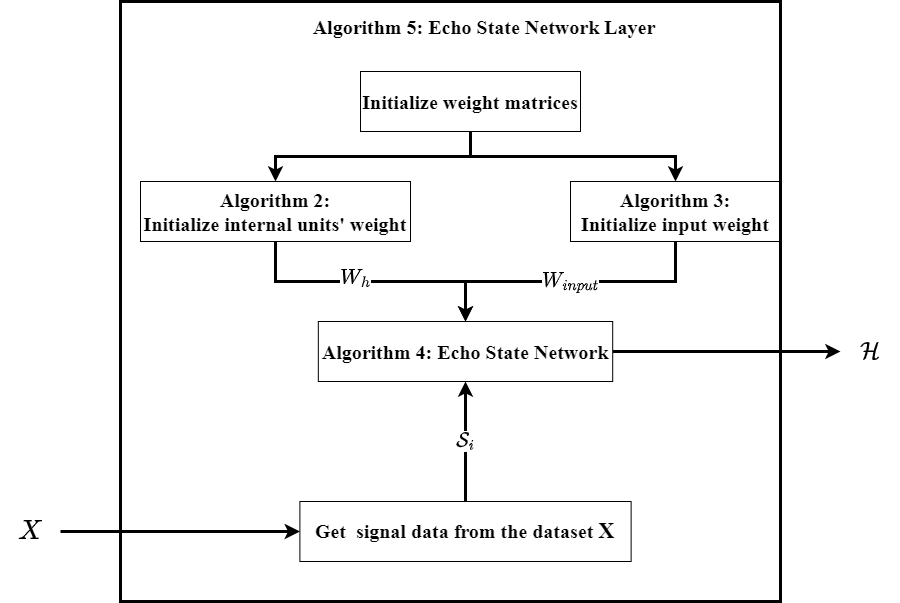
\includegraphics[width=0.95\textwidth]{img/Algorithm1.png}
    \caption{The Echo State Network layer algorithm.}
    \label{fig:Algorithm-ESN}
\end{figure}

\begin{figure}[ht]
    \centering
    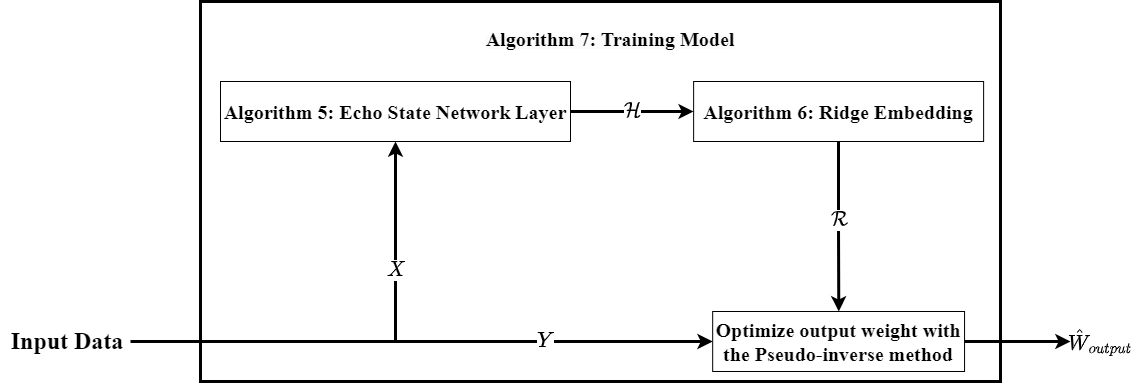
\includegraphics[width=\textwidth]{img/Algorithm2.png}
    \caption{Multi-channels Echo State Extreme
Learning Machine.}
    \label{fig:Algorithm}
\end{figure}
% Input matrix: $\mathbf{A} \in \mathbb{R}^{N \times d}$ (where $N$ is the number of training samples and $d$ is the number of features)
% Output matrix: $\mathbf{V} \in \mathbb{R}^{N \times k}$ (where $k$ is the number of output neurons)
% Hidden neuron activation function: $g(\cdot)$
% Number of hidden neurons: $l$
% \Figure[t!](topskip=0pt, botskip=0pt, midskip=0pt)[width=0.8\textwidth]{img/Algorithm1.png}
% {The Echo State Network layer algorithm.\label{Algorithm-ESN}}

% \Figure[t!](topskip=0pt, botskip=0pt, midskip=0pt)[width=0.95\textwidth]{img/Algorithm2.png}
% {Multi-channels Echo State Extreme
% Learning Machine.\label{Algorithm}}

\section{Multi-channels Echo State Extreme Learning Machine}\label{subsec:multi model}

% Reservoir computing (RC) is one of machine learning which has to learn with time series data like an RNN, but RC has a recurrent part that is fixed weight \cite{cucchi2022hands}. From the fixed recurrent weight unit weight, the RC can avoid the backpropagation process, which leads to vanishing gradient problems and consumes much time to train. Therefore, the RC has efficient learning and fast training for time series data.\\

The Multi ES-ELM model contains two parts. Figure \ref{fig:Echo-model} shows how to train Multi ES-ELM which is separated into two parts which are the fixed part and the training part. 

The first part is the ESN layer, which has fixed weight parameters and does not need a training process. The fixed weight of~ESN transforms an input signal $X$ into a hidden matrix $H$. Also, Multi ES-ELM embeds the matrix $H$ and returns Embedded vector $R$ via ridge regression embedding. 

The second part $W_{output}$ is the linear layer used to predict the label by feature data extracted from the first part\cite{cucchi2022hands, bianchi2020reservoir}. This second part is trained by the pseudo-inverse method talked about in the section ~\ref{sec:training}.

Let the matrix $W_h$ be internal recurrent units. To avoid training encoding of input time series data, The parameters $W_h$ need to follow the conditions of echo state property. There are many methods to set $W_h$ to echo state property. This research uses the methods that normalize $W_h$ by its largest absolute eigenvalue. 

The methods to initialize $W_{input}$ and $W_h$ that are shown in Algorithm \ref{init_internal}, \ref{input_weight} respectively\cite{bianchi2020reservoir, jaeger2002adaptive}. 

\begin{algorithm}
    \caption{Initialize internal units weight}
    \label{init_internal}
    \begin{algorithmic}[1]
        \renewcommand{\algorithmicrequire}{\textbf{Input:}}
        \renewcommand{\algorithmicensure}{\textbf{Output:}}
        \Require  Number of internal units $\lambda$, spectral radius $r=0.99$
    \Ensure Initialized internal weights $W_h\in\mathbb{R}^{\lambda\times\lambda}$

    \State $W_h \gets [w_{ij}]\in\mathbb{R}^{\lambda\times\lambda},\  w_{ij}\sim \mathcal{N}(0, 1)$
     
    \State $E \gets \text{eigenvalue}(W_h)$
    \State $e_{\text{max}} \gets \text{max}(\text{abs}(E))$
    \State $W_h \gets (W_h\times r) / \text{abs}(e_{\text{max}})$
    \State \textbf{return} $W_h$
    \end{algorithmic}
\end{algorithm}

\begin{algorithm}
    \caption{Initialize input weight}
    \label{input_weight}
    \begin{algorithmic}[1]
        \renewcommand{\algorithmicrequire}{\textbf{Input:}}
        \renewcommand{\algorithmicensure}{\textbf{Output:}}
        \Require Number of internal units $\lambda$, number of channels data $C = 3$
    \Ensure Initialized input weights $W_{input} \in\mathbb{R}^{\lambda\times C}$

    \State $W_{input} \gets [w_{ij}]\in\mathbb{R}^{\lambda\times C},\ w\sim U(0, 1)$
     
    \For{$i\gets 1$ \textbf{to} $\lambda$}
        \For{$j\gets 1$ \textbf{to} $C$}
            \If{$w_{ij} > 0.5$}
                \State $W_{input}[i, j]\gets 1$
            \Else
                \State $W_{input}[i, j]\gets 0$
            \EndIf
        \EndFor
    \EndFor
    \State \textbf{return} $W_{input}$
    \end{algorithmic}
\end{algorithm}

The fixed-part ESN model does not need to train but can extract the feature used to train the supervised model\cite{cucchi2022hands, bianchi2020reservoir, jaeger2002adaptive}. ESN is used to model sequential data and is governed by the RNN states equation\cite{bianchi2020reservoir}:
\begin{equation*}
    h_t = \tanh(W_{input}s_t + W_hh_{t-1})
\end{equation*}

$H = [h_1,\ldots,h_T]^\top$ is the sequence of hidden states $h_t$ generated over time and represents the encoding of signal point $s_t$ in input signal data $\mathcal{S}$. The sequence of hidden states $H$ can calculated by Algorithm \ref{ESN}.

\begin{algorithm}
    \caption{Echo State Network}
    \label{ESN}
    \begin{algorithmic}[1]
        \renewcommand{\algorithmicrequire}{\textbf{Input:}}
        \renewcommand{\algorithmicensure}{\textbf{Output:}}
        \Require Signal $\mathcal{S}\in\mathbb{R}^{C\times T}$, input weight $W_{input}\in\mathbb{R}^{\lambda\times C}$, internal weight $W_h\in\mathbb{R}^{\lambda\times\lambda}$

        \Ensure Hidden matrix $H = [h_1; h_2;,\cdots;h_{T}]$

        % \State $S \gets Signal_i$
        
        % \State $S_{input} \gets W_{input} \cdot \mathcal{S} \in\mathbb{R}^{\lambda\times T}$
        \State  $H\gets \varnothing$ 
        \State  $h_{0} \gets \mathbf{0}_{\lambda\times 1}$
        \For{$t\gets 1$ \textbf{to} $T$} 
            \State $s_{t}\gets \mathcal{S}[:, t]\in\mathbb{R}^{C\times 1}$
            \State $h_{t} \gets \tanh(W_{input}\cdot s_{t} + W_{h}\cdot h_{t-1})\in\mathbb{R}^{\lambda\times 1}$
            % \State $v\gets [v_{i}]\in\mathbb{R}^{\lambda\times1};\ v_{i}\sim\mathcal{N}(0, 1)$
            % \State $h_{t} \gets \tanh( h_{internal} + v)\in\mathbb{R}^{\lambda\times 1}$
            \State $H[t]\gets h_{t}$
            \State $h_{t-1} \gets h_{t}$

        \EndFor
    \State \textbf{return} $H\in\mathbb{R}^{\lambda\times T}$
    \end{algorithmic}
\end{algorithm}

The ridge embedding of $H$ of the ESN model is the representation of latent space ($H$) by predicting the next $n$ time steps latent state ($h_{t+n}$) from the recent latent state ($h_t$) with auto-regressive models \cite{bianchi2020reservoir}.
\begin{align*}
    % h_{t+1} &= A_th_t + B_t\\
    r_t &=  (h_t h_t^\top)^{-1} h_t h_{t+n}^\top
\end{align*}

\begin{algorithm}
    \caption{Echo State Network Layer}
    \label{ESN_layer}
    \begin{algorithmic}[1]
        \renewcommand{\algorithmicrequire}{\textbf{Input:}}
        \renewcommand{\algorithmicensure}{\textbf{Output:}}
        \Require Signal dataset $X = [\mathcal{S}_1;\mathcal{S}_2;\cdots; \mathcal{S}_N]\in\mathbb{R}^{N\times C\times T}$        

        \Ensure Set of hidden matrix $\mathcal{H} = [H_1; H_2;,\cdots;H_{N}]$
        \State $\mathcal{H}\gets\varnothing$
        \State $W_h\gets$ Algorithm \ref{init_internal} ($\lambda$)
        \State $W_{input}\gets $ Algorithm \ref{input_weight} ($\lambda,\ C$)
        
        \For{$i\gets 1$ \textbf{to} $N$}
            \State $\mathcal{H}[i] \gets$ Algorithm \ref{ESN} ($X[i],\ W_{input},\ W_h$)
        \EndFor

    \State \textbf{return} $\mathcal{H}\in\mathbb{R}^{N\times \lambda\times T}$
    \end{algorithmic}
\end{algorithm}

Ridge embedding of hidden matrix $H_i$ of input signal data $\mathcal{S}_i$ is defined by $$R_{i} = [r_1; r_2;\cdots; r_{T-n}]^\top_i$$
The Algorithm \ref{ridge} transforms hidden matrix $H_i$ to ridge embedding $R_i$. Also, for each ridge embedding $R_i$ of signal $\mathcal{S}_i$ are stacked into the list of ridge embedding $\mathcal{R}$.
$$\mathcal{R} = 
\begin{bmatrix}
    R_{1}\\ R_{2}\\ \vdots\\ R_{N}
\end{bmatrix}
$$


% \Figure[t!](topskip=0pt, botskip=0pt, midskip=0pt)[width=0.43\textwidth]{img/Echo_new.png}
% {The Echo State Network model consists of fixed part and training part.\label{Echo-model}}



\begin{algorithm}
    \caption{Ridge Embedding}
    \label{ridge}
    \begin{algorithmic}[1]
        \renewcommand{\algorithmicrequire}{\textbf{Input:}}
        \renewcommand{\algorithmicensure}{\textbf{Output:}}
        \Require Hidden spaces $H = [h_1; h_2;,\cdots;h_{T}]$, step size $n$

    \Ensure Embedded vector $R$

    % \State $X \gets [h_1; h_2;,\cdots;h_{T-n}]$ 
    % \State $y \gets [h_n; h_{n+1};,\cdots;h_{T}]$
    % \State $lhs  \gets [h_1 h_1^\top; h_2 h_2^\top;,\cdots;h_{T-n} h_{T-n}^\top]$
    % \State $rhs  \gets [h_1 h_n^\top; h_2 h_{n+1}^\top;,\cdots;h_{T-n}  h_{T}^\top]$
    \State $R\gets\varnothing$
    \For{$t\gets 1$ \textbf{to} $T-n$}
        \State $r \gets (h_t h_t^\top)^{-1} h_t h_{t+n}^\top \in\mathbb{R}^{\lambda\times\lambda}$ 
        \State $R[i] \gets flatten(r) \in\mathbb{R}^{1\times(\lambda^2)}$
    \EndFor
    \State \textbf{return} $R\in\mathbb{R}^{(T-n)\times(\lambda^2)}$
    \end{algorithmic}
\end{algorithm}

\begin{algorithm}
    \caption{Training Multi-channels Echo State Extreme Learning Machine}
    \label{multi-ESELM}
    \begin{algorithmic}[1]
        \renewcommand{\algorithmicrequire}{\textbf{Input:}}
        \renewcommand{\algorithmicensure}{\textbf{Output:}}
        \Require Signal data $X\in\mathbb{R}^{N\times C\times T}$, label data $Y\in\mathbb{R}^{N\times M}$, step size $n$
        \Ensure Optimal $\hat{W}_{output}$
        \State $\mathcal{R}\gets\varnothing$
        \State $\mathcal{H}\gets $ Algorithm \ref{ESN_layer} ($X,\ n$)
        \For{$i\gets 1$ \textbf{to} $N$} 
        \State $R \gets $ Algorithm \ref{ridge} ($\mathcal{H}[i])$
            \State $\mathcal{R}[i]\gets flatten(R)\in\mathbb{R}^{1\times(T-n)\lambda^2}$
            % \State $\mathcal{R}[i]\gets R_i$
        \EndFor
        \State $\mathcal{R}^\dagger\gets (\mathcal{R}^\top \mathcal{R})^{-1}\mathcal{R}^\top\in\mathbb{R}^{(T-n)\lambda^2\times N}$
        \State $W_{output}\gets \mathcal{R}^\dagger Y\in\mathbb{R}^{(T-n)\lambda^2\times M}$
        \State \textbf{return} $\hat{W}_{output}$
    \end{algorithmic} 
\end{algorithm}

The Multi ES-ELM model uses the list of ridge embedding $\mathcal{R}$ to be the learnable representation. The Algorithm \ref{multi-ESELM} shows how to train the Multi ES-ELM model with the input signal data $X$ and label data $Y$. The algorithm finds the optimal output weight from the list of embedding $\mathcal{R}$.  

\begin{figure}[ht]
    \centering
    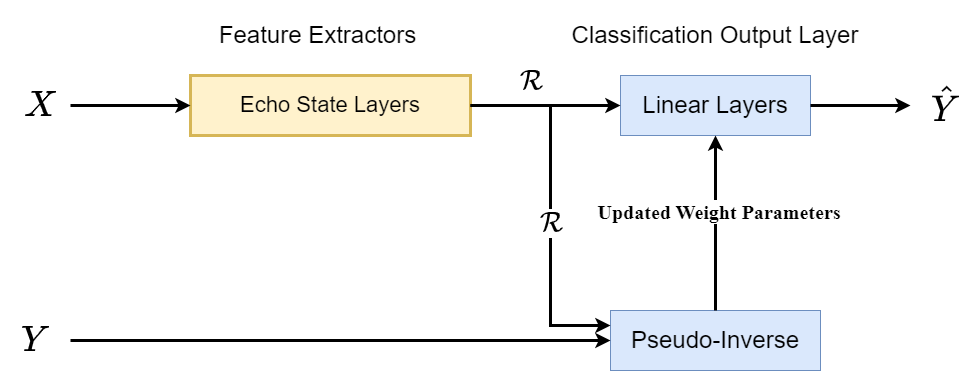
\includegraphics[width=0.95\textwidth]{img/Echo-layer.png}
    \caption{The Multi-Channel ESELM.}
    \label{fig:multi-eselm}
\end{figure}

The section \ref{sec:training} shows the pseudo-inverse method to calculate the optimal output weight $\hat{\mathcal{B}}$ of ELM. Figure \ref{fig:Algorithm} explains how the Multi ES-ELM model extracts features from data like a list of the hidden matrix $\mathcal{H}$ and a list of ridge embedding $\mathcal{R}$ that are calculated by Algorithm \ref{ESN_layer} and \ref{ridge}, the two features are calculated by the fixed part of the model. The ridge embedding $\mathcal{R}$ of the Multi ES-ELM can be compared to the ELM's hidden layer matrix $\mathbf{G}$. Thus, the optimal output weight $\hat{W}_{output}$ of Multi ES-ELM is calculated by:
$$\hat{W}_{output} = \mathcal{R}^\dagger Y$$
where $\mathcal{R}^{\dagger} = (\mathcal{R}^\top\mathcal{R})^{-1}\mathcal{R}^\top$. 
